\chapter{Обзор методов сокрытия информации} \label{chapt7}%
\textbf{Мета роботи:~}%
Изучить методы, факторы и риски при сокрытии информации.
\section{Теоретические ведомости} \label{sect6_a}
%
\textbf{Стеганография} --- это наука о передачи секретной информации, причем
сам факт передачи остаётся неизвестен внешнему наблюдателю. Развитие
стеганографии мотивируется в основном потребностью защиты интеллектуальной
собственности в компьютерных сетях, в основном в интернете.

\noindent Различают два вида стеганографии:%
\begin{Notes}
  \item  Сокрытие информации от пассивного наблюдателя. В этом случае основная цель – не
допустить обнаружения скрытой информации.
  \item  Сокрытие информации от активного противника, т.е. наличие скрытой
информации заведомо известно, но получение этой информации противником
невозможно. Этот случай распространяется на схемы защиты авторских прав.
Здесь используются digital \emph{watermarking} (цифровые водяные знаки) и
\emph{fingerprinting} (отпечатки пальцев).
\end{Notes}

\paragraph{Методы сокрытия информации}

В настоящее время методы компьютерной стеганографии развиваются по двум
основным направлениям:
\begin{enumerate}
  \item  Методы, основанные на использовании специальных свойств
      компьютерных форматов;
  \item Методы, основанные на избыточности аудио и визуальной информации.
\end{enumerate}

\subparagraph{Метод использовании свойств}
%
Здесь применяется метод использования зарезервированных для расширения полей
компьютерных форматов данных. Зарезервированные поля имеются во многих
мультимедийных форматах, они заполняются нулевой информацией и не учитываются
программой. Этот метод очень прост в использовании. Однако явным недостатком
этого метода является низкая степень скрытности и передача небольших
ограниченных объёмов информации.

Для передачи текстовых сообщений используются методы специального
форматирования текстовых файлов:

\begin{itemize}
  \item Методы, основанные на изменении положения строк и расстановки слов
      в предложении, что обеспечивается вставкой дополнительных пробелов
      между словами.
  \item Методы выбора определенных позиций букв (нулевой шифр). Акростих
      \item частный случай этого метода, когда например, начальные буквы
      каждой строки образуют сообщение или начальные буквы каждого слова.
  \item Методы, основанные на использовании специальных "невидимых",
      скрытых полей. Например, использование чёрного шрифта на чёрном фоне.
  \item Методы сокрытия в неиспользуемых местах гибких дисков. Информация
      может записываться, к примеру, на нулевую дорожку.
  \item Использования имитирующих функций (mimic-function). Метод основан
      на генерации текстов и является обобщением акростиха. Для тайного
      сообщения генерируется осмысленный текст, скрывающий само сообщение,
      расположение букв которого в сгенерированном тексте задаётся
      определённым образом.
\end{itemize}

Все эти методы просты в использовании, но малопроизводительны и обеспечивают
низкую степень скрытости. Предназначены только для передачи небольших объемов
информации.

Ярким примером применения компьютерной стеганографии является компьютерный
вирус Win95.CIH. Этот вирус внедряется в исполняемый файл *.exe. Исполняемый
файл может содержать не только код, но и многочисленные дополнительные
данные: пиктограммы, различные служебные данные и информация об
экспортируемых и импортируемых функциях. Каждый вид данных, содержащихся в
файле, это отдельный объект, занимающий секцию фиксированного размера. Если
объект не занимает всего объёма секции, то эта часть секции не используется.
Поэтому в файле формата РЕ всегда достаточно свободного места для записи.

\subparagraph{Метод избыточности информации}
%
Младшие разряды представления аудио и видео формата малоинформативны и их
изменение практически не сказывается на качестве передаваемого изображения
или звука, что дает возможность использования их для кодирования
конфиденциальной информации. Но при введении дополнительной информации
искажаются статистические характеристики передаваемого файла, что может
привести к обнаружению передаваемого сообщения. Для повышения устойчивости к
обнаружению применяют методы коррекции статистических характеристик. Основным
достоинством данного метода является возможность скрытой передачи большого
объёма информации, а также возможность защиты авторского права, скрытого
изображения товарной марки, регистрационных номеров и т.п.

Наиболее распространенным является метод замены наименее значимых битов или
LSB метод. Суть этого подхода заключается в том , что за счет погрешности
дискретизации изменение младших разрядов в аудио видео изображении
практически не сказывается на качестве передаваемого звука или картинки,
особенно если изначально оно было закодировано с большой глубиной передачи
цвета. Визуально определить было ли изображение подвергнуто трансформации или
нет невозможно, но, используя специальные методы, основанные на
статистическом анализе, можно сказать, было ли вкраплено в файл некоторое
дополнительное количество информации и даже извлечь ее.

Другие популярные методы встраивания секретных сообщений основаны на
использовании форматов файлов с потерей данных (например, JPEG). В отличие от
LSB методов они более стойки к геометрическим преобразованиям и обнаружению
канала передачи. Это достигается за счет возможности изменять качество сжатых
данных в широком диапазоне, что приводит к невозможности определения
происхождения изображения.

В современных системах формирования цифровых водяных знаков используется
принцип встраивания метки, являющейся узкополосным сигналом, в то время как
само маркируемое изображение является широкополосным. Указанный метод
реализуется при помощи двух основных алгоритмов и их модификаций. В первом из
них используется фазовая модуляция сигнала с псевдослучайной
последовательностью чисел для сокрытия секретной информации. Во втором случае
весь канал передачи информации делится на несколько каналов и передача
осуществляется между ними. На плане исходного изображения встраиваемая метка
представляет из себя дополнительный шум со своими статистическими
характеристиками. За счет того, что некоторый шум в изображениях присутствует
всегда, встраивание метки влияет лишь на уровень имеющегося шума, обычно
незаметного для органов чувств. Кроме всего метка является устойчивой к
выделению из основного сигнала за счет ее рассеивания по всему частотному
диапазону изображения.

\paragraph{Примеры методов звуковых файлов}
%
\textbf{Low-bit coding}. Является самым простым метод встроить метку в
структуру данных. Наименее значимые биты в самплах заменяются на биты
встраиваемой метки. Основным недостатком этого метода является его слабая
устойчивость к манипуляциям над файлом. В процессе ресамплинга или в
результате передачи скрытое сообщение может быть легко искажено или вообще
потеряно.

\textbf{Phase Coding} заменяет фазу оригинального звукового сегмента на
относительную фазу, которая и представляет собой секретное сообщение. Фаза
последовательных сегментов добавляется таким образом, чтобы сохранить
относительный фазовый сдвиг между сегментами. Phase coding – один из наиболее
эффективных методов сокрытия информации  в терминах отношения уровня сигнала
к заметному искажению этого сигнала. Когда отношение фаз между частотами
сильно меняется, происходит заметная фазовая дисперсия. Однако “неслышное”
кодирование при этом все равно достигается, так как изменение фазы достаточно
мало.

\textbf{Spread spectrum}. В обычном канале связи стремятся сконцентрировать
информацию в как можно более узком диапазоне частот, чтобы сохранить
доступную полосу пропускания и уменьшить энергию, необходимую для передачи.
Основной метод расширения спектра спроектирован таким образом, чтобы
закодировать поток информации, распространяя секретные данные в как можно
большем спектре частот. Это позволяет извлечь скрытую в потоке информацию,
даже если происходит интерференция на некоторых частотах.

\textbf{Echo data hiding}. При использовании этого метода данные заключаются
в оригинальный звуковой сигнал посредством ввода эха. Данные скрываются при
помощи изменения трех параметров эха: начальной амплитудой, степени затухания
и задержки.  Когда задержка между оригинальным сигналом и эхом уменьшается,
сигналы смешиваются. В некоторой точке человеческое ухо уже не может
различить эти два сигнала, эхо ощущается как добавочный резонанс. Эту точку
достаточно сложно определить, она зависит о качества оригинальной записи,
типа записи и слушателя. Обычно слияние сигналов осуществляется в районе
1/1000 секунды, что характерно для большинства типов звуков и слушателей. При
кодировании используется две временные задержки, одна для обозначения
логической единицы (\emph{offset}), другая для логического нуля (offset +
delta). Обе задержки должны быть меньше порога чувствительности человеческого
уха, при котором он может обнаружить эхо. Вдобавок к уменьшению временной
задержки необходимо убедиться, что информацию нельзя раскрыть установлением
начальной амплитуды и степени затухания ниже порога слышимости человеческого
уха.

Для улучшения характеристик сигнала при использовании различных методов
сокрытии информации в медиаданных, а также повышения устойчивости полученного
сигнала к его анализу и обнаружению скрытой информации применяются некоторые
полезные дополнения к обычным алгоритмам стеганографии. Вот некоторые из них.

\textbf{Adaptive data attenuation}. Оптимальный фактор подстройки изменяется
при изменении уровня оригинального сигнала. Адаптируя подстройку к небольшим
изменениям уровня сигнала или шума, можно удерживать уровень сигнала,
представляющего закодированные данные, очень низким в течение интервалов
тишины и увеличивать во время интервалов большего уровня звука.

\textbf{Redundancy and error correction coding}. Для того чтобы избежать
ошибок при получении сигнала вследствие шума в канале или изменении
оригинального звука, полезно применять кодирование с исправлением ошибок к
скрываемым данным. Тем не менее, при использовании алгоритмов коррекции
ошибок приходиться обходиться компромиссным вариантом, учитывающим надежность
данных и объём данных, которые можно при этом скрыть.

\textbf{Sound context analysis}. Обнаруживаемость белого шума, встроенного в
оригинальный сигнал, линейно зависит от уровня первоначального звука. Для
максимизации объёма скрываемых данных, при условии, что они не будут
обнаружены, полезно измерять уровень шума при кодировании. Уровень шума можно
определить, измеряя изменение амплитуды сигнала в близлежащих самплах.

\subparagraph{Стохастическая модуляция}

Одним из последних методов стеганографии является прием стохастической
модуляции. На примере графического файла он представляется следующим образом.

Сообщение, которое необходимо передать, обозначим $m$, состоящее из
последовательных $1$ и $-1(логический 0)$. Сначала определяется вероятностная
функция $P(x,s) \in {-1,1}$, равная $0$ только при $s=0$. Она также должна
удовлетворять свойству антисимметричности для всех $x: P(x+s,s)=-P(x-s,s)$.
Это свойство полезно в тех случаях, когда значения x+s или x-s выходят за
допустимый диапазон значений. При наложении секретной информации пикселы
проходятся в псевдослучайной последовательности, построенной с помощью
генератора случайных чисел с  распределением, совпадающим с распределением
шума, который будет наложен на  картинку. Такая последовательность называется
стегошумом. При генерации используется специальный стегоключ. Для каждой
точки x генерируется случайной число s. Если s отлично от нуля, то если
$P(x+s,s)=m$, то значение пикселя заменяется на $x+s$, если $P(x+s,s)=-m$, то
значение заменяется на $x-s$. Формально процесс сокрытия есть
\begin{equation}\label{eq:7_1}
x'_i=xi+m_i \cdot P(x_i+s_i,s_i)\cdot s_i
\end{equation}

Так как само изображение и стегошум $s_i$ не зависят от секретного сообщения,
то сигнал $v_i=m_i \cdot P(x_i+s_i,s_i)$ является псевдослучайной
последовательностью $1$ и $-1$. Таким образом, $v_i$ имеет такие же
статистические свойства, что и стегошум.

Для извлечения закодированного сообщения генерируется стегошум по тому же
стегоключу, что и при кодировании. Применяя вероятностную функцию $P$ к
пикселам изображения, получаем секретное сообщение, формируемое из ненулевых
значений $m_i = P(x_i,s_i)$.

В рассмотренном выше методе используется только один стегошум $s_i$, который
добавляется или вычитается из значений пикселя в соответствии с вероятностной
функцией. Возможно получить больший объём скрываемой информации с теми же
шумовыми характеристиками.

\emph{Улучшенный метод стохастической модуляции} использует сразу два
стегошума, добавляя к значениям пикселей изображения всегда либо один
стегошум, либо другой, основываясь опять на совпадении бит сообщения и
вероятностной функции. Этот метод работает для стегошума с произвольным
вероятностным распределением.

Метод стохастической модуляции можно также применять для изображений,
полученных с помощью устройств, шум которых зависит от содержания
изображения. Подробно этот способ рассмотрен в
\todo{[2]}. %%% [2]	Digital image steganography using stochastic modulation, Jessica Fridrich and Miroslav Goljan, 2003 http://www.ws.binghamton.edu/fridrich/Research/stochastic_modulation02.pdf






\subparagraph{Использование шума}
%
Есть два конечных абонента, которые хотят совершить разговор на расстоянии, с
помощью какого-нибудь канала связи. Сам канал они не контролируют. Необходимо
избежать утечки информации путем кодирования.

Для решения этой проблемы используется наложение защитного шума
(накладывается шум перед отдачей в канал связи, и соответственно снимается
перед выводом на динамик). Шум должен быть случайным или, что то же самое,
белым (большинство источников генерируют псевдо-случайный шум — такой шум
достаточно легко может быть подавлен).

При использовании остальных способов шифрования остаются остаточные признаки
речи, по которым, обладая достаточно мощным вычислительным комплексом, можно
получить исходную речь в приемлемом качестве.

Даже если использовать белый шум возникают проблемы: его так же надо
как-нибудь передать адресату, иначе (если не передавать), то злоумышленник
может сделать то же самое, что и адресат (подавить шум).

\subparagraph{Шум для шифрования изображений}

Визуальная криптография впервые была введена Мони Наором и Ади Шамиром в 1994
году. Она используется для шифрования изображения или текста, представленного
в виде изображения. Основная идея модели визуальной криптографии состоит в
разбиении исходного изображения на несколько шифрованных («теневых»
изображений, shadow images), каждое из которых не дает никакой информации об
исходном изображении кроме, может быть, его размера (изображение – а-ля
«белый шум»). При наложении шифрованных изображений друг на друга, можно
получить исходное изображение. Таким образом, для декодирования не требуется
специальных знаний, высокопроизводительных вычислений и даже компьютера (в
случае, если распечатать теневые изображения на прозрачных пленках). В случае
использования этого алгоритма в компьютерных системах, наложить все части
изображения друг на друга можно используя логические операции AND, OR, XOR
(или установив более высокую степень прозрачности в графическом редакторе).
Данная технология обладает криптоустойчивостью за счёт того, что при
разделении исходного изображения на множество шифроизображений происходит
случайным образом.

\begin{figure} [htbp]
  \centering
  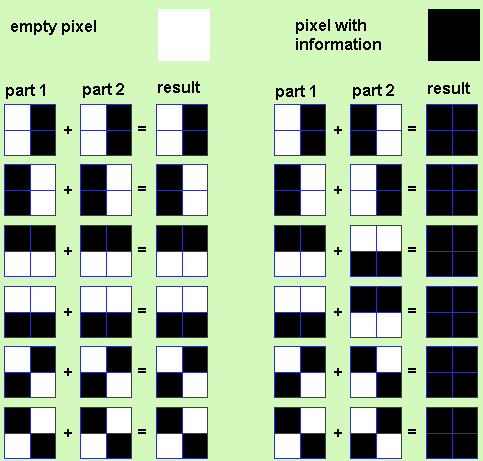
\includegraphics[width=\linewidth]{prSostojania}
  \caption{Возможные состояния пикселя при визуальной схеме $2x2$}\label{img7x1}
\end{figure}


\paragraph{Методы обнаружения информации}
 Обнаружения информации в файлах.

\textbf{Rarjpeg} --- это особый вид файлов, представляющий собой склеенную
вплотную jpeg-картинку и rar-архив. Он является прекрасным контейнером для
сокрытия передачи информации. Создать rarjpeg можно с помощью следующих
команд:%

\begin{lstlisting}
  UNIX: cat image1.jpg archive.rar > image2.jpg
  WINDOWS: copy /b image1.jpg+archive.rar image2.jpg
  Или же при наличии hex-редактора.
\end{lstlisting}

Разумеется, для скрытия факта передачи информации можно использовать не
только формат JPEG, но и многие другие. Каждый формат имеет свои особенности,
благодаря которым он может подходить или нет для роли контейнера.

\paragraph{Методы детектирования склеенных файлов}
\subparagraph{Метод проверки области после EOF-маркера} Множество популярных
форматов файлов имеют так называемый маркер конца файла, который отвечает за
отображение нужных данных. Например, программы для просмотра фотографий
считывают все байты вплоть до этого маркера, однако, область после него
остается игнорируемой. Этот метод идеально подходит для форматов: JPEG, PNG,
GIF, ZIP, RAR, PDF.

\subparagraph{Метод проверки размера файла} Структура некоторых форматов
(аудио- и видеоконтейнеры) позволяет вычислить реальный размер файла и
сравнить его с исходным размером. Форматы: AVI, WAV, MP4, MOV.

\subparagraph{Метод проверки CFB-файлов} CFB или Compound File Binary Format
— формат документов, разработанный в Microsoft, представляющий собой
контейнер с собственной файловой системой. Этот метод основан на обнаружении
аномалий в файле.

\subparagraph{Продолжение файла}

Ознакомившись с предыдущими тегами можно сделать вывод, что данные в файл
могут быть записаны и после основного содержимого.

Далее предоставим несколько примеров:

\textbf{JPEG}

Для нахождения ответа на этот вопрос, необходимо углубиться в спецификации
формата, который является «родоначальником» склеенных файлов и понять его
структуру. Любой JPEG начинается с сигнатуры 0xFF 0xD8.

После этой сигнатуры находится служебная информация, опционально иконка
изображения и, наконец, само сжатое изображение. В этом формате конец
изображения отмечается двухбайтной сигнатурой 0xFF 0xD9.

\textbf{PNG}

Первые восемь байт PNG-файла занимает следующая сигнатура: 0x89, 0x50, 0x4E,
0x47, 0x0D, 0x0A, 0x1A, 0x0A. Сигнатура конца, которая заканчивает поток
данных: 0x49, 0x45, 0x4E, 0x44, 0xAE, 0x42, 0x60, 0x82.

\textbf{RAR}

Общая сигнатура для всех rar-архивов: 0x52 0x61 0x72 0x21 (Rar!). После неё
идет информация о версии архива и прочие сопутствующие данные. Опытным путём
было установлено, что архив заканчивается сигнатурой 0x0A, 0x25, 0x25, 0x45,
0x4F, 0x46.

\begin{table} [htbp]% Пример записи таблицы с номером, но без отображаемого наименования
  \centering
  %\parbox{6cm}{% чтобы лучше смотрелось, подбирается самостоятельно
    \caption{Таблица форматов и сигнатур RAR}%
    \label{tabl:tab7x1}%
    \begin{SingleSpace}
      \begin{tabularx}{\textwidth}{|c|L|L|}
      \hline
      Формат & Начальная сигнатура & Конечная сигнатура \tabularnewline \hline
      JPEG   & 0xFF 0xD8                                & 0xFF 0xD9                               \tabularnewline \hline
      PNG    & 0x89 0x50 0x4E 0x47 0x0D 0x0A 0x1A 0x0A  & 0x49 0x45 0x4E 0x44 0xAE 0x42 0x60 0x82 \tabularnewline \hline
      RAR    & 0x52 0x61 0x72 0x21                      & 0x0A 0x25 0x25 0x45 0x4F 0x46           \tabularnewline \hline
      \end{tabularx}
    \end{SingleSpace}
\end{table}

Алгоритм проверки на склейку в данных форматах предельно прост:
\begin{enumerate}
\item Найти начальную сигнатуру;
\item Найти конечную сигнатуру;
\item Если после конечной сигнатуры нет данных --- ваш файл чист и не
    содержит вложений! В ином случае необходимо искать после конечной
    сигнатуры другие форматы.
\end{enumerate}

\textbf{GIF} и \textbf{PDF}

\begin{table} [htbp]% Пример записи таблицы с номером, но без отображаемого наименования
  \centering
    \captiondelim{ } % разделитель идентификатора с номером от наименования
    \caption{}%
    \label{tabl:tab7x2}%
    \begin{SingleSpace}
      \begin{tabularx}{\textwidth}{|c|L|L|}
        \hline
        Формат & Начальная сигнатура & Конечная сигнатура             \tabularnewline \hline
        GIF    & 0x47 0x49 0x46 0x38 & 0x00 0x3B                      \tabularnewline \hline
        PDF    & 0x25 0x50 0x44 0x46 & 0x0A 0x25 0x25 0x45 0x4F 0x46  \tabularnewline \hline
      \end{tabularx}
    \end{SingleSpace}
\end{table}




PDF документ может иметь более одного EOF-маркера, например, из-за
неправильной генерации документа. Количество конечных сигнатур в GIF-файле
равно количеству кадров в нём. Исходя из особенностей этих форматов, можно
улучшить алгоритм проверки наличия приклеенных файлов.
\begin{enumerate}
  \item Пункт 1 повторяется из предыдущего алгоритма.
  \item Пункт 2 повторяется из предыдущего алгоритма.
  \item При нахождении конечной сигнатуры запомнить её расположение и искать дальше;
  \item Если таким образом дошли до последнего EOF-маркера — файл чист.
  \item Если файл не заканчивается конечной сигнатурой — goto место последней найденной конечной сигнатуры.
\end{enumerate}

Большая разница между размером файла и позицией после последней конечной
сигнатуры указывает на наличие приклеенного вложения. Разница может
составлять больше десяти байт, хотя возможна установка иных значений.

\textbf{ZIP}

Особенность ZIP-архивов заключается в наличие трех различных сигнатур:

\begin{table} [htbp]% Пример записи таблицы с номером, но без отображаемого наименования
  \centering
  \parbox{14cm}{% чтобы лучше смотрелось, подбирается самостоятельно
    \captiondelim{ } % разделитель идентификатора с номером от наименования
    \caption{}%
    \label{tabl:tab7x3}%
    \begin{SingleSpace}
      \begin{tabular}{|l|l|}
      \hline
      Сигнатуры           & Описание                                \\ \hline
      0x50 0x4B 0x03 0x04 & Сигнатура обычного архива               \\ \hline
      0x50 0x4B 0x05 0x06 & Сигнатура пустого архива                \\ \hline
      0x50 0x4B 0x07 0x08 & Сигнатура архива, разделенного на части \\ \hline
      \end{tabular}
    \end{SingleSpace}
    }
\end{table}


\begin{table} [htbp]% Пример записи таблицы с номером, но без отображаемого наименования
  \centering
  \parbox{6cm}{% чтобы лучше смотрелось, подбирается самостоятельно
    \captiondelim{ } % разделитель идентификатора с номером от наименования
    \caption{ }%
    \label{tabl:tab7x4}%
    \begin{SingleSpace}
      \begin{tabular}{|l|}
      \hline
      {Local File Header 1}       \\ \hline
      {File Data 1}               \\ \hline
      {Data Descriptor 1}         \\ \hline
      {Local File Header 2}       \\ \hline
      {File Data 2}               \\ \hline
      {Data Descriptor 2}         \\ \hline
      ...                                             \\ \hline
      {Local File Header n}       \\ \hline
      {File Data n}               \\ \hline
      {Data Descriptor n}         \\ \hline
      {Archive decryption header} \\ \hline
      {Archive extra data record} \\ \hline
      {Central directory}         \\ \hline
      \end{tabular}
    \end{SingleSpace}
    }
\end{table}

Больше всего интересна центральная директория, которая содержит метаданные о
файлах в архиве. Центральная директория всегда начинается с сигнатуры 0x50
0x4b 0x01 0x02 и заканчивается сигнатурой 0x50 0x4b 0x05 0x06, после которых
следует 18 байт метаданных. Что интересно, пустые архивы состоят только из
конечной сигнатуры и 18 нулевых байт. После 18 байт следует область
комментария к архиву, которая является идеальным контейнером для скрытия
файла.

Для проверки ZIP-архива необходимо найти конечную сигнатуру центральной
директории, пропустить 18 байт и искать сигнатуры известных форматов в
области комментария. Большой размер комментария также свидетельствует о факте
склейки.

\textbf{AVI}

Структура AVI-файла следующая: каждый файл начинается с сигнатуры RIFF (0x52
0x49 0x46 0x46). На 8 байте идет уточняющая формат сигнатура AVI (0x41 0x56
0x49 0x20). Блок на смещении 4, состоящий из 4 байт, содержит начальный
размер блока данных (порядок байт — little endian). Чтобы узнать номер блока,
содержащего следующий размер, необходимо сложить размер заголовка (8 байт) и
размер, полученный в блоке 4-8 байт. Таким образом вычисляется полный размер
файла. Допускается, что вычисленный размер может быть меньше, чем реальный
размер файла. После вычисленного размера файл будет содержать только нулевые
байты (необходимо для выравнивания границы в 1 Кб).

\begin{figure}[htbp]
  \centering
  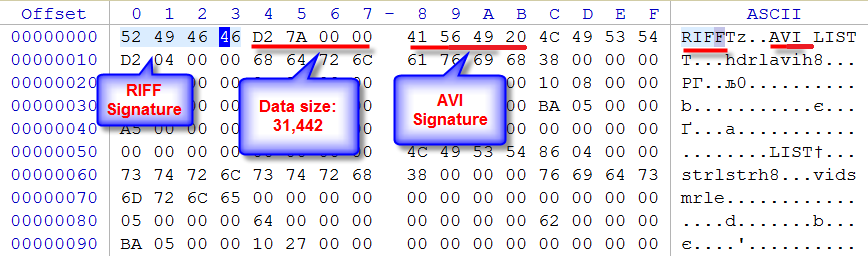
\includegraphics[width=\linewidth]{img7x1}
  \caption{Пример вычисления AVI}\label{img7x2}
\end{figure}

\textbf{WAV}

Как и AVI, WAV-файл начинается с сигнатуры RIFF, однако, у этого файла
сигнатура с 8 байта — WAVE (0x57 0x41 0x56 0x45). Размер файла вычисляется
таким же образом, как и AVI. Реальный размер должен полностью совпадать с
вычисленным.

 \textbf{MP4}

MP4 или MPEG-4 – формат медиаконтейнера, используемый для хранения видео- и
аудиопотоков, также предусматривает хранение субтитров и изображений.

На смещении 4 байта расположены сигнатуры: тип файла ftyp (66 74 79 70)
(QuickTime Container File Type) и подтип файла mmp4 (6D 6D 70 34). Для
распознания скрытых файлов, нас интересует возможность вычисления размера
файла.

\begin{figure}[htbp]
  \centering
  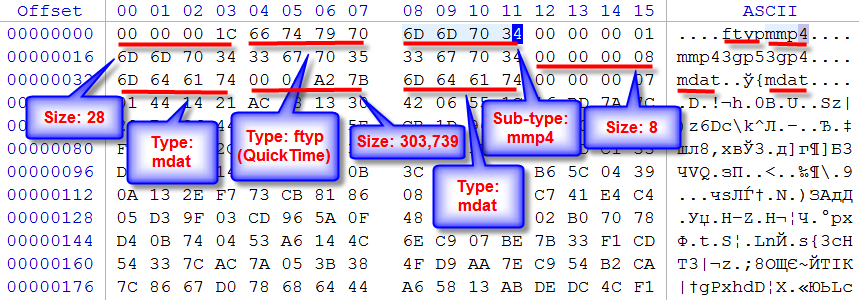
\includegraphics[width=\linewidth]{img7x3}
  \caption{Пример вычисления MP4}\label{img:img7x3}
\end{figure}


Рассмотрим пример. Размер первого блока находится на нулевом смещении, и он
равен 28 (00 00 00 1С, порядок байт Big Endian); он же указывает на смещение,
где находится размер второго блока данных. На 28 смещении находим следующий
размер блока равный 8 (00 00 00 08). Чтобы найти следующий размер блока,
необходимо складывать размеры найденных предыдущих блоков.

Таким образом, вычисляется размер файла:
\begin{table} [htbp]% Пример записи таблицы с номером, но без отображаемого наименования
  \centering
  %\parbox{6cm}{% чтобы лучше смотрелось, подбирается самостоятельно
    \captiondelim{ } % разделитель идентификатора с номером от наименования
    %\caption{Структура ZIP архива }%
    \label{tabl:tab7x5}%
    \begin{SingleSpace}
      \begin{tabular}{|l|l|l|}
      \hline
      Смещение & Значение & Следующее смещение \\ \hline
      0        & 28       & 28+0=28            \\ \hline
      28       & 8        & 28+8=36            \\ \hline
      36       & 303739   & 36+303739=303775   \\ \hline
      303775   & 6202     & 303775+6202=309977 \\ \hline
      \end{tabular}
    \end{SingleSpace}
\end{table}

\textbf{MOV}

Этот широко используемый формат является также контейнером MPEG-4. MOV
использует проприетарный алгоритм сжатия данных, имеет похожую на MP4
структуру и используется в тех же целях — для хранения аудио и видеоданных, а
также сопутствующих материалов.

Как и MP4, любой mov-файл имеет на 4 смещении 4-х байтную сигнатуру ftyp,
однако, следующая сигнатура имеет значение qtyp (71 74 20 20). Правило
вычисления размера файла не изменилось: начиная с начала файла вычисляем
размер следующего блока и складываем.

Метод проверки этой группы форматов на наличие «приклеенных» файлов
заключается в вычислении размера по заданным выше правилам и сравнении его с
размером проверяемого файла. Если текущий размер файла много меньше
вычисленного, то это указывает на факт склейки. При проверке AVI-файлов
допускается, что вычисленный размер может быть меньше размера файла из-за
наличия добавленных нулей для выравнивания границы. В таком случае,
необходимо проверять нули после вычисленного размера файла.


\section{Задания}\label{sect6_b}
Цель практической части работы состоит в получении \todo{максимально коэф.}
сокрытия информации.
%
\begin{enumerate}
  \item Изучить теорию, быть готовым к опросу.
  \item Сокрыть информацию с помощью предоставленного ПО: %
  \begin{enumerate}
    \item в тесте;
    \item в изображении;
    \item в музыке.
  \end{enumerate}
  \item Сравнение методов и выводы к работе.
\end{enumerate}
\section{Инструкция к работе с ПО}\label{sect6_c}
%
(ф-ции программы, методы и т.д.)
\section{Вопросы для контроля}\label{sect6_e}
%
\begin{enumerate}
  \item Какие есть способы сокрытия информации?
  \item В каких файлах лучше скрывать информацию?
  \item Что такое шум?
  \item Риски потери и дешифровка информации.
\end{enumerate}
